\section{preparation}
\subsection{What are the three basic components of the laser?}
\begin{itemize}
    \item Gas filling \\
    \to mixture of helium and neon in a ratio of 5:1
    \item Pump source \\
    \to electric discharger which imparts energy to the gas atoms
    \item optical Resonator \\
    \to two mirrors, one partially reflecting and one fully reflecting
\end{itemize}
\subsection{What defines the wavelength of a laser?}
\begin{itemize}
    \item emitted energy of the photon corresponding to the energydifference 
    of the electrons
\end{itemize}
\subsection{Discuss the most important process in the active medium 
(absorption, stimulated emission and spontaneous emission).}
\begin{itemize}
    \item Absorption \\
    \to electron jumps to excited state 
    \item Spontaneous emission \\
    \to electron returns to lower state ands emit a random, incoherent photon
    \item Stimulated emission \\
    \to a photon encounters an excited atom and stimulates it to emit a coherent 
    photon which the same energy and direction
\end{itemize}
\begin{figure}
    \centering
    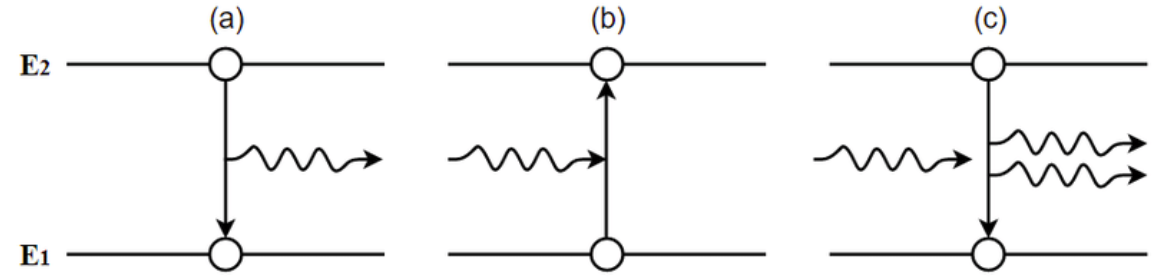
\includegraphics{pictures/emission.png}
\end{figure}

\subsection{Discuss the relationship between the amplification of 
the light and the population inversion in the active medium}
\begin{itemize}
    \item Population inversion is necessary for stimulated emission to dominate
    \item more particles are in the exited state than in the groundstate
    \item stimulated emission leads to the amplification of light
\end{itemize}

\subsection{Why is a two-level laser not possible?}
\begin{itemize}
    \item population inversion is not possible
    \item absorption and spontaneous emission are equally likely $B_{12}=B_{21}$
    \item domination of stimulated emission is not possible
\end{itemize}

\subsection{Which transition is responsible for the red line of the He-Ne laser?}
\begin{itemize}
    \item Neon transition $\text{5s}\to\text{3p}$ with $\SI{632.8}{\nano\meter}$
\end{itemize}

\subsection{How is the population inversion achieved?}
\begin{itemize}
    \item Electrical Discharge \\
    \to electrical voltage generates a discharge in the gas mixture, raising the energy of helium atoms
    \item Collisions \\
    \to excited helium atoms collide with neon atoms, transfering their energy \\
    \to neon atoms absorb energy 
\end{itemize}

\subsection{Calculate the stability parameters $g_1\cdot g_2$ as a function of the 
resonant length $L$ for at least two resonator configurations and plot the result}
\subsection{What is the maximum resonator length that can be achieved?}

\subsection{Describe the intensity curve in the plane perpendicular to the 
propagation direction for $\text{TEM}_{00}$ and $\text{TEM}_{01}$.}
\begin{itemize}
    \item $\text{TEM}_{00}$ \\
    \to a single, symmetric peak around the center 
    \item $\text{TEM}_{01}$\\
    \to two intensity peaks around the center
\end{itemize}
\begin{figure}
    \centering
    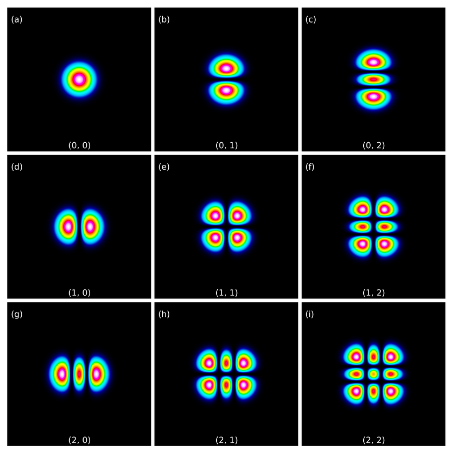
\includegraphics{pictures/TEM.png}
    \label{fig:TEM}
\end{figure}

\subsection{Explain the term "intracavity aperture for mode selection".}
\begin{itemize}
    \item component within the laser to control the lasers's output mode
\end{itemize}
\subsection{What is the difference between longitudinal and transversal modes?}
\begin{itemize}
    \item longitudinal \\
    \to Variation of wavelength along the laser resonator axis
    \item transversal \\
    \to Spatial distribution of light intensity in a plane perpendicular to the axis
\end{itemize}

\subsection{Describe the broadening of the optical transition in gas due to the Doppler effect.}
\subsection{How large is the spectral boardening for the optical transition in 
Ne gas at room temperature?}
\subsection{Describe the mode spectrum (frequency spectrum) for the laser with 
typical resonator length $L=\SI{1.5}{\meter}$.}
\subsection{How does mode selection work with the help of Fabry-Perot etalon?}

\subsection{The laser under investigation is equipped with Brewster windows fitted
to the laser tubes. What is the role of the Brewster windows?}
\subsection{What is the resulting polarisation of the laser?}